\documentclass[aspectratio=169,11pt]{beamer}

\usepackage{fontspec}
\setmainfont{PT Serif}
\setsansfont{PT Sans}
\setmonofont{PT Mono}
\usepackage{polyglossia}
\setmainlanguage{russian}
\setotherlanguage{english}
\newfontfamily\cyrillicfonttt{PT Mono}

\usepackage{amsmath,amssymb,mathtools}
\usepackage{graphicx}
\usepackage{booktabs}
\usepackage{animate}
\usepackage{hyperref}
\usepackage{tikz}
\usepackage[backend=biber,style=numeric,sorting=none]{biblatex}
\IfFileExists{tex/references.bib}{\addbibresource{tex/references.bib}}{\addbibresource{references.bib}}

\usetheme{default}
\usefonttheme{professionalfonts}
\useinnertheme{rounded}
\setbeamertemplate{navigation symbols}{}
\setbeamertemplate{caption}[numbered]
\graphicspath{{assets/}{../assets/}}

% Calm, consistent visual style.
\definecolor{nsgaNavy}{HTML}{203864}
\definecolor{nsgaBlue}{HTML}{2F75B5}
\definecolor{nsgaLight}{HTML}{F4F7FB}
\definecolor{nsgaGreen}{HTML}{5B9B72}
\definecolor{nsgaOrange}{HTML}{D98E32}
\setbeamercolor{normal text}{fg=black,bg=white}
\setbeamercolor{structure}{fg=nsgaBlue}
\setbeamercolor{frametitle}{fg=white,bg=nsgaNavy}
\setbeamercolor{title}{fg=nsgaNavy}
\setbeamercolor{block title}{fg=white,bg=nsgaBlue}
\setbeamercolor{block body}{fg=black,bg=nsgaLight}
\setbeamercolor{exampleblock title}{fg=white,bg=nsgaGreen}
\setbeamercolor{exampleblock body}{fg=black,bg=nsgaLight}
\setbeamercolor{alertblock title}{fg=white,bg=nsgaOrange}
\setbeamercolor{alertblock body}{fg=black,bg=nsgaLight}
\setbeamertemplate{itemize item}{\color{nsgaBlue}$\blacktriangleright$}
\setbeamertemplate{enumerate item}{\color{nsgaBlue}\insertenumlabel.}
\setbeamertemplate{frametitle}{%
  \nointerlineskip\begin{beamercolorbox}[wd=\paperwidth,ht=0.78cm,dp=0.22cm,leftskip=0.45cm]{frametitle}%
    \usebeamerfont{frametitle}\insertframetitle
  \end{beamercolorbox}}
\setbeamertemplate{footline}{%
  \hfill\scriptsize\color{nsgaNavy}\insertframenumber/\inserttotalframenumber\hspace{0.35cm}\vspace{0.18cm}}
\setbeamersize{text margin left=0.55cm,text margin right=0.55cm}

% Image helpers: fixed safe boxes, no stretching, no clipping.
\newcommand{\fitimage}[1]{%
  \includegraphics[width=0.90\linewidth,height=0.64\textheight,keepaspectratio]{#1}}
\newcommand{\wideimage}[1]{%
  \includegraphics[width=0.96\linewidth,height=0.72\textheight,keepaspectratio]{#1}}
\newcommand{\halfimage}[1]{%
  \includegraphics[width=0.44\linewidth,height=0.42\textheight,keepaspectratio]{#1}}
\newcommand{\twocolimage}[1]{%
  \includegraphics[width=0.98\linewidth,height=0.44\textheight,keepaspectratio]{#1}}
\newcommand{\animfront}[1]{%
  \animategraphics[autoplay,loop,controls,width=0.78\textwidth,height=0.54\textheight,keepaspectratio]{8}{#1/frame_}{000}{024}}

\title[NSGA-II]{Быстрый элитарный многокритериальный генетический алгоритм}
\subtitle{Non-dominated Sorting Genetic Algorithm~--- версия~II \\
\small Deb, Pratap, Agarwal, Meyarivan~--- IEEE TEC, 2002}
\author{Ластовецкий Дмитрий}
\institute{Университет ИТМО\\Институт математики}
\date{2026}

\begin{document}

% ─────────────────────────────────────────────────────────────────────────────
\begin{frame}
  \titlepage
\end{frame}

% ─────────────────────────────────────────────────────────────────────────────
\begin{frame}{Парето-доминирование и фронт Парето}
  \begin{block}{Доминирование \hfill $\displaystyle\min_{x \in D}\;(f_1(x),\ldots,f_M(x))$}
    $x \prec y \;\iff\;
    \bigl(\forall i:\; f_i(x) \le f_i(y)\bigr)
    \;\land\;
    \bigl(\exists j:\; f_j(x) < f_j(y)\bigr)$
  \end{block}
  \vspace{0.15cm}
  \begin{exampleblock}{}
    \textbf{Парето-оптимальное решение}~--- никто из популяции его не доминирует;
    улучшить по одному критерию нельзя без ухудшения другого.\\
    \textbf{Фронт Парето}~--- множество всех таких точек в пространстве целей.
  \end{exampleblock}
  \vspace{0.1cm}
  \begin{columns}
    \column{0.48\textwidth}
      \centering \halfimage{zdt1_true_front.png}
      {\footnotesize ZDT1: выпуклый фронт}
    \column{0.48\textwidth}
      \centering \halfimage{zdt3_true_front.png}
      {\footnotesize ZDT3: разрывный фронт (5 кусков)}
  \end{columns}
\end{frame}

% ─────────────────────────────────────────────────────────────────────────────
% ─────────────────────────────────────────────────────────────────────────────
\begin{frame}{Первый NSGA: как он работал}\small
  \begin{exampleblock}{Srinivas и Deb (1994)}
    Сначала разложить популяцию на недоминируемые фронты, затем присвоить особям из лучших фронтов больший \textbf{фитнес}~--- числовую оценку качества~--- и размножать их генетическими операторами.
  \end{exampleblock}
  \vspace{0.15cm}
  \begin{columns}[T]
    \column{0.50\textwidth}
      \textbf{Схема одного поколения:}
      \begin{enumerate}\footnotesize
        \item Найти первый недоминируемый фронт $\mathcal{F}_1$.
        \item Удалить его, найти $\mathcal{F}_2$, потом $\mathcal{F}_3$ и так далее.
        \item Назначить фитнес по рангу фронта: чем лучше ранг, тем выше оценка.
        \item Внутри фронта применить ниширование (sharing): штраф за слишком плотную толпу соседей.
        \item Сделать отбор, скрещивание и мутацию.
      \end{enumerate}
    \column{0.46\textwidth}
      \begin{alertblock}{Три слабости}
        \begin{itemize}\footnotesize
          \item сортировка $O(MN^3)$;
          \item нет элитизма: хорошая точка может пропасть;
          \item нужен ручной параметр ниширования~--- радиус $\sigma_{\mathrm{share}}$.
        \end{itemize}
      \end{alertblock}
      \footnotesize
      Здесь $N$~--- размер популяции, $M$~--- число целевых функций.
  \end{columns}
\end{frame}

% ─────────────────────────────────────────────────────────────────────────────
\begin{frame}{Три нововведения NSGA-II}
  \large
  \begin{enumerate}
    \item \textbf{Быстрая недоминируемая сортировка:}\\
          $O(MN^3) \;\to\; O(MN^2)$ \quad\small($N$~--- особей в популяции, $M$~--- целей)\\
          \normalsize При $N{=}100,\,M{=}2$: $\;2\,000\,000 \to 20\,000$ операций.

    \vspace{0.4cm}
    \item \textbf{Расстояние толпы} (\textit{crowding distance}):
          автоматическая оценка «незаполненности» окрестности каждой точки~---
          без параметров.

    \vspace{0.4cm}
    \item \textbf{Оператор сравнения $\prec_n$:}
          единый критерий отбора: ближе к фронту + уникальнее.
  \end{enumerate}
\end{frame}

% ─────────────────────────────────────────────────────────────────────────────
\begin{frame}{Недоминируемые фронты: что это?}
  \begin{exampleblock}{}
    Разбиваем популяцию на «слои»:
    \textbf{Ранг 1}~--- лучшие (никто из популяции их не доминирует).
    \textbf{Ранг 2}~--- лучшие из оставшихся. И т.\,д.
    Меньший ранг = ближе к фронту Парето.
  \end{exampleblock}
  \vspace{0.2cm}
  \centering
  \begin{tikzpicture}[scale=0.88]
    \draw[->] (0,0) -- (5,0) node[right] {$f_1$};
    \draw[->] (0,0) -- (0,3.5) node[above] {$f_2$};
    \foreach \x/\y in {0.4/2.8, 0.9/2.1, 1.6/1.5, 2.5/1.0, 3.6/0.5} {
      \fill[blue!70] (\x,\y) circle(4pt);
    }
    \draw[blue!50,dashed,thick] (0.4,2.8) -- (0.9,2.1) -- (1.6,1.5) -- (2.5,1.0) -- (3.6,0.5);
    \node[blue!80,right,font=\small] at (3.6,0.5) {\textbf{Ранг 1} $\mathcal{F}_1$};
    \foreach \x/\y in {0.7/3.3, 1.5/2.5, 2.6/1.8, 3.8/1.2} {
      \fill[orange!80] (\x,\y) circle(4pt);
    }
    \node[orange!80,right,font=\small] at (3.8,1.2) {\textbf{Ранг 2} $\mathcal{F}_2$};
    \foreach \x/\y in {1.2/3.2, 2.3/2.8, 3.5/2.2} {
      \fill[red!60] (\x,\y) circle(4pt);
    }
    \node[red!80,right,font=\small] at (3.5,2.2) {\textbf{Ранг 3} $\mathcal{F}_3$};
  \end{tikzpicture}
\end{frame}

% ─────────────────────────────────────────────────────────────────────────────
\begin{frame}{Быстрая недоминируемая сортировка}
  \textbf{Для каждой особи $p$ запоминаем:}
  \begin{itemize}
    \item $n_p$~--- сколько особей \emph{лучше} $p$ (доминируют над ней);
    \item $S_p$~--- список особей, которых $p$ \emph{сама доминирует}.
  \end{itemize}
  \vspace{0.15cm}
  \footnotesize
  \begin{enumerate}
    \item Сравнить все пары → заполнить $n_p$ и $S_p$.
    \item $\mathcal{F}_1 = \{p : n_p = 0\}$ (никто не лучше~--- это ранг 1).
    \item Для каждой $p \in \mathcal{F}_1$, для каждой $q \in S_p$:
          уменьшить $n_q$ на 1. Если $n_q = 0$ → $q$ в $\mathcal{F}_2$.
    \item Повторять для $\mathcal{F}_2, \mathcal{F}_3,\ldots$ до конца.
  \end{enumerate}
  \normalsize
  \vspace{0.2cm}
  \begin{alertblock}{Почему $O(MN^2)$?}
    Двойной цикл: $N(N-1)/2$ пар, каждое сравнение $O(M)$.
    При $N=100, M=2$: $\approx 10\,000$ операций.
    Старый NSGA с $O(MN^3)$: $\approx 2\,000\,000$.
  \end{alertblock}
\end{frame}

% ─────────────────────────────────────────────────────────────────────────────
\begin{frame}{Расстояние толпы~--- зачем?}\small
  \begin{exampleblock}{}
    На одном и том же ранге нужно предпочитать \textbf{более уникальные}
    решения~--- те, что находятся в разреженных частях фронта.
    Иначе все точки стянутся в одну кучу.
  \end{exampleblock}
  \vspace{0.2cm}
  \centering
  \begin{tikzpicture}[scale=0.66]
    \draw[->] (0,0) -- (5.5,0) node[right] {$f_1$};
    \draw[->] (0,0) -- (0,3.5) node[above] {$f_2$};
    \draw[blue!40,thick] (0.55,3.05) .. controls (1.3,2.10) and (2.6,1.15) .. (5.0,0.68);
    \fill[red!70] (0.55,3.25) circle(4pt);
    \fill[red!70] (4.8,0.7) circle(4pt);
    \foreach \x/\y in {1.9/1.73,2.0/1.65,2.1/1.56,2.2/1.48,2.3/1.42} {
      \fill[green!70] (\x,\y) circle(4pt);
    }
    \fill[orange!80] (1.0,3.3) circle(5.5pt)
      node[above right,orange!80,font=\small] {выгоднее: пусто вокруг};
    \fill[gray!60] (2.1,1.56) circle(5.5pt)
      node[below right,gray!60,font=\small] {невыгодно: толпа};
    \node[font=\small,blue!60] at (4.05,2.15) {фронт $\mathcal{F}_1$};
  \end{tikzpicture}
\end{frame}

% ─────────────────────────────────────────────────────────────────────────────
\begin{frame}{Расстояние толпы~--- иллюстрация}
  \centering
  \wideimage{crowding_illustration.png}
  \vspace{0.08cm}
  {\footnotesize
    Для каждой точки $i$: нормированное расстояние до соседей слева и справа.
    Крайним точкам~--- $\infty$ (их выбирать всегда выгодно).
  }
\end{frame}

% ─────────────────────────────────────────────────────────────────────────────
\begin{frame}{Расстояние толпы~--- формула}
  \textbf{Алгоритм} для фронта $\mathcal{I}$ из $l$ точек:
  \begin{enumerate}
    \item Всем: $i_{\mathrm{dist}} = 0$.
    \item Для каждого критерия $m$:
      \begin{itemize}
        \item Отсортировать по $f_m$.
        \item Крайним: $i_{\mathrm{dist}} = \infty$.
        \item Остальным прибавить:
        \[
          i_{\mathrm{dist}} \mathrel{+}=
          \frac{f_m\bigl(\mathcal{I}[i{+}1]\bigr) - f_m\bigl(\mathcal{I}[i{-}1]\bigr)}
               {f_m^{\max} - f_m^{\min}}.
        \]
      \end{itemize}
  \end{enumerate}
  \begin{alertblock}{Физический смысл}
    $i_{\mathrm{dist}}$~--- периметр прямоугольника, построенного на ближайших соседях.
    Большой периметр = точка в «незаполненном» месте = ценная.
  \end{alertblock}
\end{frame}

% ─────────────────────────────────────────────────────────────────────────────
\begin{frame}{Оператор сравнения с толпой $\prec_n$}
  \begin{exampleblock}{}
    Как выбрать лучшего из двух кандидатов?\\[4pt]
    1. У кого меньший ранг (ближе к фронту)~--- тот лучше.\\
    2. Если ранги одинаковы~--- лучше тот, у кого \emph{больше}
       расстояние толпы (в менее заполненном месте).
  \end{exampleblock}
  \vspace{0.3cm}
  \begin{block}{Формально}
    $i \prec_n j$
    $\iff$
    $\begin{cases}
       i_{\mathrm{rank}} < j_{\mathrm{rank}}, \\[4pt]
       i_{\mathrm{rank}} = j_{\mathrm{rank}}
         \;\land\;
         i_{\mathrm{dist}} > j_{\mathrm{dist}}.
    \end{cases}$
  \end{block}
  \vspace{0.2cm}
  В \textbf{бинарном турнире}: случайно берём двух особей,
  побеждает лучший по $\prec_n$.
\end{frame}

% ─────────────────────────────────────────────────────────────────────────────
\begin{frame}{Элитизм~--- как реализован}
  \begin{exampleblock}{}
    Перед отбором \emph{объединяем} родителей $P_t$ и потомков $Q_t$.
    Из объединения $R_t = P_t \cup Q_t$ (размер $2N$) выбираем лучшие $N$.
    Если ни один потомок не лучше родителя~--- родитель остаётся.
    Хорошие решения \textbf{гарантированно не теряются}.
  \end{exampleblock}
  \vspace{0.3cm}
  \centering
  \begin{tikzpicture}[scale=0.85]
    \node[draw,fill=blue!15,rounded corners,minimum width=2cm,minimum height=0.9cm]
      (P) at (0,0) {$P_t$\;\small($N$ особей)};
    \node[draw,fill=orange!15,rounded corners,minimum width=2cm,minimum height=0.9cm]
      (Q) at (0,-1.5) {$Q_t$\;\small(потомки, $N$)};
    \node[draw,fill=purple!10,rounded corners,minimum width=2.6cm,minimum height=0.9cm]
      (R) at (3.8,-0.75) {$R_t = P_t \cup Q_t$\;\small($2N$)};
    \node[draw,fill=green!15,rounded corners,minimum width=2cm,minimum height=0.9cm]
      (P2) at (7.5,-0.75) {$P_{t+1}$\;\small(лучшие $N$)};
    \draw[->,thick] (P.east) -- (R.west);
    \draw[->,thick] (Q.east) -- (R.west);
    \draw[->,thick] (R) -- node[above,font=\small]{сортировка} (P2);
  \end{tikzpicture}
\end{frame}

% ─────────────────────────────────────────────────────────────────────────────
\begin{frame}{Главный цикл NSGA-II}
  \footnotesize
  \begin{tabular}{p{0.53\textwidth}p{0.42\textwidth}}
    \toprule
    \textbf{Шаг} & \textbf{Что происходит} \\
    \midrule
    $R_t = P_t \cup Q_t$
      & Объединить родителей и потомков → $2N$ особей \\[4pt]
    $\mathcal{F} = \texttt{fast-non-dominated-sort}(R_t)$
      & Разбить $R_t$ на ранги $\mathcal{F}_1, \mathcal{F}_2, \ldots$ \\[4pt]
    Добавлять $\mathcal{F}_1, \mathcal{F}_2,\ldots$ в $P_{t+1}$
      & Брать целые фронты, пока не наполним $N$ мест \\[4pt]
    Последний фронт: сортировать по $\downarrow i_{\mathrm{dist}}$
      & Из «пограничного» фронта взять самые уникальные \\[4pt]
    $Q_{t+1} = \texttt{make-new-pop}(P_{t+1})$
      & Турнир $\to$ скрещивание $\to$ мутация \\
    \bottomrule
  \end{tabular}
\end{frame}

% ─────────────────────────────────────────────────────────────────────────────
\begin{frame}{Схема одного поколения}
  \centering
  \wideimage{nsga2_procedure.png}
\end{frame}

% ─────────────────────────────────────────────────────────────────────────────
\begin{frame}{Как создаются потомки: SBX и мутация}
  \begin{exampleblock}{SBX (Simulated Binary Crossover~--- симулированное бинарное скрещивание)}
    Берём двух родителей и создаём двух потомков, находящихся «вокруг» родителей.
    Параметр $\eta_c$: большой~--- потомки близко к родителям (точный поиск);
    малый~--- далеко (широкий поиск). В статье: $\eta_c = 20$.
  \end{exampleblock}
  \vspace{0.3cm}
  \begin{exampleblock}{Полиномиальная мутация}
    Случайное малое изменение одной переменной потомка с вероятностью $p_m = 1/n$.
    Позволяет исследовать точки, недостижимые только скрещиванием.
    В статье: $\eta_m = 20$.
  \end{exampleblock}
\end{frame}

% ─────────────────────────────────────────────────────────────────────────────
\begin{frame}{Сложность~--- что значит $O(MN^2)$}
  \begin{exampleblock}{Обозначения}
    $N$~--- размер популяции, то есть сколько решений сравниваем в одном поколении.\\
    $M$~--- число целевых функций, например цена/качество/вес дают $M=3$.
  \end{exampleblock}
  \vspace{0.08cm}
  \begin{exampleblock}{}
    $O(MN^2)$ означает: количество операций $\approx M \times N^2$.\\
    При удвоении $N$ работа растёт в 4 раза.
    У старого NSGA ($O(MN^3)$): в 8 раз~--- т.\,е. в $N$ раз медленнее.
  \end{exampleblock}
  \vspace{0.2cm}
  \begin{tabular}{llll}
    \toprule
    Шаг & Сложность & При $N=100, M=2$ \\
    \midrule
    Быстрая сортировка & $O(MN^2)$ & $\approx 20\,000$ оп. \\
    Расстояние толпы & $O(MN\log N)$ & $\approx 1\,300$ оп. \\
    Отбор из $\mathcal{F}_l$ & $O(N\log N)$ & $\approx 700$ оп. \\
    \midrule
    \textbf{Итого} & $\boldsymbol{O(MN^2)}$ & $\approx 20\,000$ оп. \\
    \midrule
    NSGA (старый) & $O(MN^3)$ & $\approx 2\,000\,000$ оп. \\
    \bottomrule
  \end{tabular}
\end{frame}

% ─────────────────────────────────────────────────────────────────────────────
\begin{frame}{Тестовые функции: что такое ZDT1, ZDT2, ZDT3}\scriptsize
  \renewcommand{\arraystretch}{1.13}
  ZDT~--- стандартный набор синтетических задач Zitzler--Deb--Thiele. Они нужны не ради прикладного смысла, а чтобы проверить алгоритм на фронтах разной формы.
  \vspace{0.12cm}
  \begin{tabular}{p{0.10\textwidth}p{0.08\textwidth}p{0.16\textwidth}p{0.56\textwidth}}
    \toprule
    \textbf{Задача} & \textbf{$n$} & \textbf{Фронт} & \textbf{Зачем нужна} \\
    \midrule
    SCH (Schaffer) & 1 & простой выпуклый & Игрушечная проверка: две цели $x^2$ и $(x-2)^2$, истинный фронт легко увидеть. \\
    ZDT1 & 30 & выпуклый & Базовый тест: надо свести $x_2,\ldots,x_n$ к нулю и равномерно покрыть гладкую кривую. \\
    ZDT2 & 30 & невыпуклый & Проверяет, не «проваливается» ли метод на вогнутом участке фронта. \\
    ZDT3 & 30 & разрывный & Самый наглядный пример: фронт состоит из нескольких отдельных островков, алгоритм должен найти все. \\
    ZDT4 & 10 & много локальных ловушек & Проверяет устойчивость к ложным фронтам: легко застрять далеко от истинного решения. \\
    \bottomrule
  \end{tabular}
  \vspace{0.12cm}
  \footnotesize
  Во всех ZDT первые координаты задают форму фронта, а функция $g(x_2,\ldots,x_n)$ штрафует уход от настоящего фронта. Поэтому алгоритм должен одновременно приблизиться к фронту и распределиться по нему равномерно.
\end{frame}

% ─────────────────────────────────────────────────────────────────────────────
\begin{frame}{Структура ZDT: как устроены функции}\small
  \textbf{Общая форма:}\quad
  $f_1 = x_1$,\quad
  $f_2 = g(x_2,\ldots,x_n)\cdot h(f_1,\,g)$,\quad
  $x_i \in [0,1]$, $n=30$.

  \smallskip
  $g$ штрафует за отклонение «лишних» переменных $x_2,\ldots,x_n$ от нуля.
  На истинном фронте $g = 1$.
  \vspace{0.15cm}

  \renewcommand{\arraystretch}{1.4}
  \begin{tabular}{p{0.11\textwidth}p{0.40\textwidth}p{0.38\textwidth}}
    \toprule
    & $g(x_2,\ldots,x_n)$ & $h(f_1,g)$ \\
    \midrule
    \textbf{ZDT1}
      & $\displaystyle 1 + \frac{9}{n-1}\sum_{i=2}^{n} x_i$
      & $1 - \sqrt{f_1/g}$ \newline{\footnotesize выпуклый фронт} \\
    \textbf{ZDT2}
      & то же
      & $1 - (f_1/g)^2$ \newline{\footnotesize невыпуклый фронт} \\
    \textbf{ZDT3}
      & то же
      & $1 - \sqrt{f_1/g} - \dfrac{f_1}{g}\sin(10\pi f_1)$
        \newline{\footnotesize $\sin$ создаёт 5 разрывных кусков} \\
    \midrule
    \textbf{SCH}
      & \multicolumn{2}{l}{$n=1$,\quad $f_1=x^2$,\quad
        $f_2=(x-2)^2$,\quad $x\in[-10^3,\,10^3]$} \\
    \bottomrule
  \end{tabular}
\end{frame}

% ─────────────────────────────────────────────────────────────────────────────
\begin{frame}{ZDT1: эволюция~--- поколение за поколением}
  \centering
  \small
  $n=30,\; N=100,\; T=250,\; \eta_c=\eta_m=20$

  \footnotesize цвет = ранг (синий~--- ранг 1; красный~--- хуже)
  \vspace{0.1cm}

  \animfront{frames_zdt1}
\end{frame}

% ─────────────────────────────────────────────────────────────────────────────
\begin{frame}{ZDT2: невыпуклый фронт}
  \centering
  \small
  $n=30,\; N=100,\; T=250$

  \footnotesize без ручных параметров алгоритм строит невыпуклую кривую
  \vspace{0.1cm}

  \animfront{frames_zdt2}
\end{frame}

% ─────────────────────────────────────────────────────────────────────────────
\begin{frame}{ZDT3: разрывный фронт}
  \centering
  \small
  $n=30,\; N=100,\; T=250$

  \footnotesize алгоритм самостоятельно «находит» все пять кусков фронта
  \vspace{0.1cm}

  \animfront{frames_zdt3}
\end{frame}

% ─────────────────────────────────────────────────────────────────────────────
\begin{frame}{Финальные результаты}
  \centering
  \wideimage{final_fronts.png}
\end{frame}


% ─────────────────────────────────────────────────────────────────────────────
\begin{frame}{NSGA против NSGA-II: одинаковые функции}\small
  \begin{columns}[T]
    \column{0.50\textwidth}
      \centering
      \twocolimage{compare_zdt1.png}
      {\footnotesize ZDT1: NSGA-II ближе и ровнее покрывает фронт.}
    \column{0.50\textwidth}
      \centering
      \twocolimage{compare_zdt3.png}
      {\footnotesize ZDT3: NSGA-II лучше удерживает отдельные куски фронта.}
  \end{columns}
  \vspace{0.08cm}
  {\scriptsize Серые линии~--- истинный фронт, точки~--- найденный первый фронт после одинакового бюджета вычислений.}
\end{frame}

% ─────────────────────────────────────────────────────────────────────────────
\begin{frame}{Почему NSGA-II выигрывает визуально}\small
  \begin{columns}[T]
    \column{0.48\textwidth}
      \begin{block}{У NSGA}
        \begin{itemize}\footnotesize
          \item без элитизма хорошие точки могут исчезнуть;
          \item ниширование зависит от ручного параметра $\sigma_{\mathrm{share}}$;
          \item сортировка дороже, поэтому при том же времени меньше полезных поколений.
        \end{itemize}
      \end{block}
    \column{0.48\textwidth}
      \begin{exampleblock}{У NSGA-II}
        \begin{itemize}\footnotesize
          \item родители и потомки конкурируют вместе, лучшие сохраняются;
          \item crowding distance держит точки разнесёнными;
          \item $O(MN^2)$ вместо $O(MN^3)$.
        \end{itemize}
      \end{exampleblock}
  \end{columns}
  \vspace{0.12cm}
  \centering
  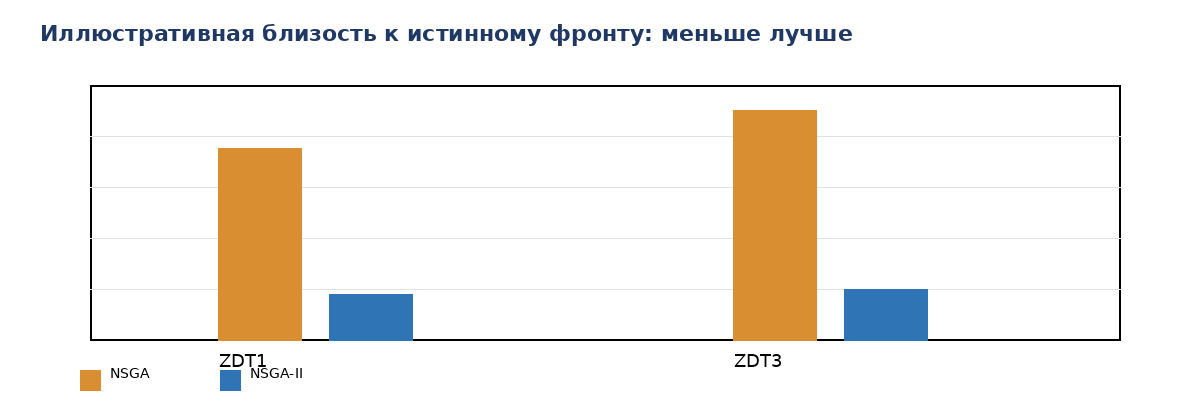
\includegraphics[width=0.74\textwidth,height=0.36\textheight,keepaspectratio]{compare_metrics.png}
\end{frame}

% ─────────────────────────────────────────────────────────────────────────────
\begin{frame}{Как измерять качество}
  \normalsize
  \textbf{Метрика сходимости} $\Upsilon$~--- насколько найденный фронт \emph{близко}
  к истинному.
  \[
    \Upsilon = \frac{1}{|H|}
      \sum_{h \in H} \min_{x \in \hat{\mathcal{F}}} \|h - x\|_2.
  \]
  $H$~--- эталонные точки на истинном фронте. \textbf{Меньше~--- лучше. $\Upsilon=0$~--- точно на фронте.}

  \vspace{0.18cm}
  \textbf{Метрика разнообразия} $\Delta$~--- насколько \emph{равномерно} распределены точки.
  \[
    \Delta = \frac{d_f + d_l + \sum_{i=1}^{N-1}|d_i - \bar{d}|}
                  {d_f + d_l + (N-1)\bar{d}}.
  \]
  $d_i$~--- расстояния между соседними точками. \textbf{$\Delta=0$~--- идеальная равномерность.}
\end{frame}

% ─────────────────────────────────────────────────────────────────────────────
\begin{frame}{Кривые сходимости и разнообразия}
  \centering
  \wideimage{convergence_diversity.png}
\end{frame}

% ─────────────────────────────────────────────────────────────────────────────
\begin{frame}{Сравнение: NSGA и NSGA-II}\small
  \renewcommand{\arraystretch}{1.18}
  \begin{tabular}{p{0.22\textwidth}p{0.33\textwidth}p{0.33\textwidth}}
    \toprule
    & \textbf{NSGA} & \textbf{NSGA-II}\\
    \midrule
    Сортировка & $O(MN^3)$ & $O(MN^2)$\\
    Элитизм & нет: найденная хорошая точка может потеряться & да: выбираем лучших из $P_t \cup Q_t$\\
    Разнообразие & ниширование (fitness sharing) с ручным $\sigma_{\mathrm{share}}$ & расстояние толпы без параметров\\
    Выбор между точками & фитнес после ниширования & ранг + расстояние толпы, оператор $\prec_n$\\
    Практический эффект & медленнее, чувствительнее к настройкам & точнее сходится к фронту, равномернее его покрывает\\
    \bottomrule
  \end{tabular}
  \vspace{0.18cm}
  \footnotesize
  $N$~--- число особей в популяции, $M$~--- число целевых функций. NSGA-II устраняет три слабости предшественника: медленная сортировка, отсутствие элитизма и ручной параметр ниширования~\cite{deb2002nsga2}.
\end{frame}

% ─────────────────────────────────────────────────────────────────────────────
\begin{frame}{Что гарантировано, а что нет}
  \large
  \textbf{Гарантировано:}
  \begin{itemize}
    \item Лучшее найденное решение не ухудшается от поколения к поколению.
    \item При достаточном числе поколений алгоритм, как правило,
          находит хорошее приближение к фронту Парето.
  \end{itemize}
  \vspace{0.3cm}
  \textbf{Не гарантировано:}
  \begin{itemize}
    \item Точное нахождение \emph{всего} фронта Парето~--- только вероятностно.
    \item Одинаковый результат при разных запусках (алгоритм случайный).
  \end{itemize}
  \vspace{0.3cm}
  \normalsize
  \textbf{Теорема «No Free Lunch»} \cite{wolpert1997nofree}: не существует
  алгоритма, лучшего на всех задачах сразу.
\end{frame}

% ─────────────────────────────────────────────────────────────────────────────
\begin{frame}{Итоги}
  \large
  \begin{enumerate}
    \item NSGA-II решает 3 проблемы NSGA: скорость, элитизм, параметр нишинга.
    \vspace{0.2cm}
    \item $O(MN^2)$~--- при $N=100$ это в 100 раз меньше операций, чем $O(MN^3)$.
    \vspace{0.2cm}
    \item Расстояние толпы~--- разнообразие без ручной настройки.
    \vspace{0.2cm}
    \item Оператор $\prec_n$ совмещает качество (ранг) и уникальность.
    \vspace{0.2cm}
    \item По сравнению с первым NSGA он быстрее, устойчивее и лучше сохраняет найденный фронт.
  \end{enumerate}
\end{frame}

% ─────────────────────────────────────────────────────────────────────────────
\begin{frame}{Код}
  \centering
  \Large
  \texttt{notebooks/nsga2\_demo.ipynb}
  \vspace{0.6cm}
  \normalsize
  \begin{tabular}{ll}
    Ядро алгоритма   & \texttt{src/nsga2\_core.py} \\
    Эксперименты     & \texttt{notebooks/nsga2\_demo.ipynb} \\
    Анимации и графики & \texttt{scripts/generate\_assets.py} \\
  \end{tabular}
\end{frame}

% ─────────────────────────────────────────────────────────────────────────────
\begin{frame}[allowframebreaks]{Литература}
  \tiny
  \printbibliography
\end{frame}

\end{document}
